\chapter{Visualisation implementation of the Improved Kepler Visualisation Tool (IKVT)}\label{C:sd}
This chapter discusses the implementation of the visulisation using the designs
discussed in the previous chapter to fullfil the requirements for this project. It details the tools used, the deliverable features
produced, and the problems encountered. IKVT displays all 2234 exoplanets
in the Kepler exoplanets dataset ((REF[28]))~ datase. Each of these exoplanets are represented as coloured
ellipses, of which the colour and size are representative of the exoplanets
temperature and size respectively. IKVT displays all of these exoplanets as if
they are orbiting a single star which in reality would result in planetary
collisions but in the visualisation provides users with a way to effectively
make observations and comparisions about each of the exoplanets in a single
view. 

To make this selection, a user can click on any of the orbiting exoplanets.  A
further effect of this selection is that a text box will have further textual
information about the selected exoplanet appended to it to provide the user with
more detailed information. When a user is unable to accurately select an exoplanet due to clustering or
overlapping of exoplanets they can move the camera around in space to gain a
better viewing position with which to make their selection. If this is not
enough, the user can use a set of range filters to filter the exoplanets
displayed. These filters are Kepler Object of Interest number (KOI),
temperature, size, and Earth Similarity Index (ESI). These filters allow for
users to fine tune the exoplanets they wish to see which allows them to work
with small multiples rather than the entire dataset.

In addition to the orbital view already discussed, there is a graph view taht
displays the exoplanets on a graph with the exoplanet attributes mapping to the
x,y coordinates. This allows the user to modify what they want on each axis of
the graph. Having these two views allows the user the option of how they wish to
visualise the exoplanets, the less exact and more visually appealing orbital
view, or the more exact and less exiting graph view.

There are two panels that make up the visualisation, the visualisation panel,
and the control panel. The visualisation panel is where all of the exoplanets
are displayed as well as text boxes describing the state of the visualisation to
keep the user informed. The control panel contains all of the interactive
components that the user can use to change the state of the visualisation. The
components it contains are; two text areas that cane be used interchangably to
display information about selected planets, four range sliders that are used to
filter the exoplanets as discused previously, and eight buttons to toggle the
state of the visualisations. These buttons are "Sort by KOI", "Sort by Temp",
"Sort by Size", "Sort by ESI", "Change View", "Suns Habitable Zone", "Pause",
and "Unsort". ~

The Kepler Orrery visualisation as discussed in the Existing Systems section of
Chapter 3 details a contrasting system that displays each exoplanet and its
sister planets orbiting its own star. By incorporating this idea into IKVT, when
a planet is selected it should be highlighted and all of its sister planets
should also become hightlighted. This will provide the same effect as in the
Kepler Orrery.  

\section{Additional Tools and artifacts used}
\subsection{Dataset used}
The dataset for this project is a comma seperated values file (CSV) that
contains all of the data pertaining to the Exoplanets. At runtime this dataset
is read into the system and an Exoplanet object is created for each element and
contains all of the information from the dataset record.

%possibly discuss how a real database could be used instead
\subsection{Integrated Development Environment (IDE)}
The IDE used for this project is one that is provided with Processing. This IDE
provided all of the tools and functionality that were required to effectively
implement the solution for this project. Another option that could have been
taken was to use Eclipse with the processing package and external libraries
imported. However I found that the processing IDE was entirely suitable for the
majority of my needs creating the visualisation. The key things that I did not
have access to with this choice was the Eclipse Debugger and JUnit tests. ~   
\subsection{Keyboard and Mouse System}
In addition to Processing in the main system there was an additional opensource
library required for effective user interface components, this library was
called ControlP5 REF~. This library is a customisable and intuitive interactive
user interface. It allows for easy creation of visually appealing and precisely
layed out interactive GUI components.

\subsection{Microft Kinect sensor system}
For the version of the IKVT system that uses the Kinect sensor for user
interaction two additional libraries were required to integrate the hardware
with Processing, these were:
\begin{enumerate}
 \item NITE
http://www.primesense.com/news/our-blog/the-dld-experience/attachment/photo4/~
 \item SimpleOpenNi http://code.google.com/p/simple-openni/~
\end{enumerate}
These libraries provided drivers to run the Kinect sensor in Processing as well
as basic gesture recognition and body tracking. However as the libraries were
opensource due to the official Microsoft Kinect SDK not being compatible with
Processing, the gesture recognition was not as user friendy or effective as the
official libraries. The effect of this was that the gesture tracking used in the
system had to be created supoptimally from the opensource libraries. 

\section{Main interface components}
The visualisation was designed to emphasis small multiples and filtering of the
Exoplanets to display the information more clearly to users.

However I will need to ensure the effectiveness of the visualisation does not
become diminished by trying to convey to much information which would lead to
cluttering and overlapping in the visualisation, as well as information overload
for users. There will also be larger emphasis placed on making the existing
system more usable by improving the interaction methods for users. The following
list outlines the new requirements for the visualisation being developed. This
will be done by providing GUI elements for each form of interaction with the
system, as well as ensuring all interaction methods are intuitive for users. 

\subsubsection{Spacial arrangement of components}
As the majority of the interaction and movement of visualisation elements occurs
in the center of the window it caused a aspect ratio that was not suitable . It
was BETTER~ to use 2 vertical columns to view and control the visualisation as
it had a higher aspect ratio which allowed more of the content to be seen on the
screen at once thanks to the fact that the majority of computer screens have a
wide ratio.

\begin{figure}[h!]
  \centering
      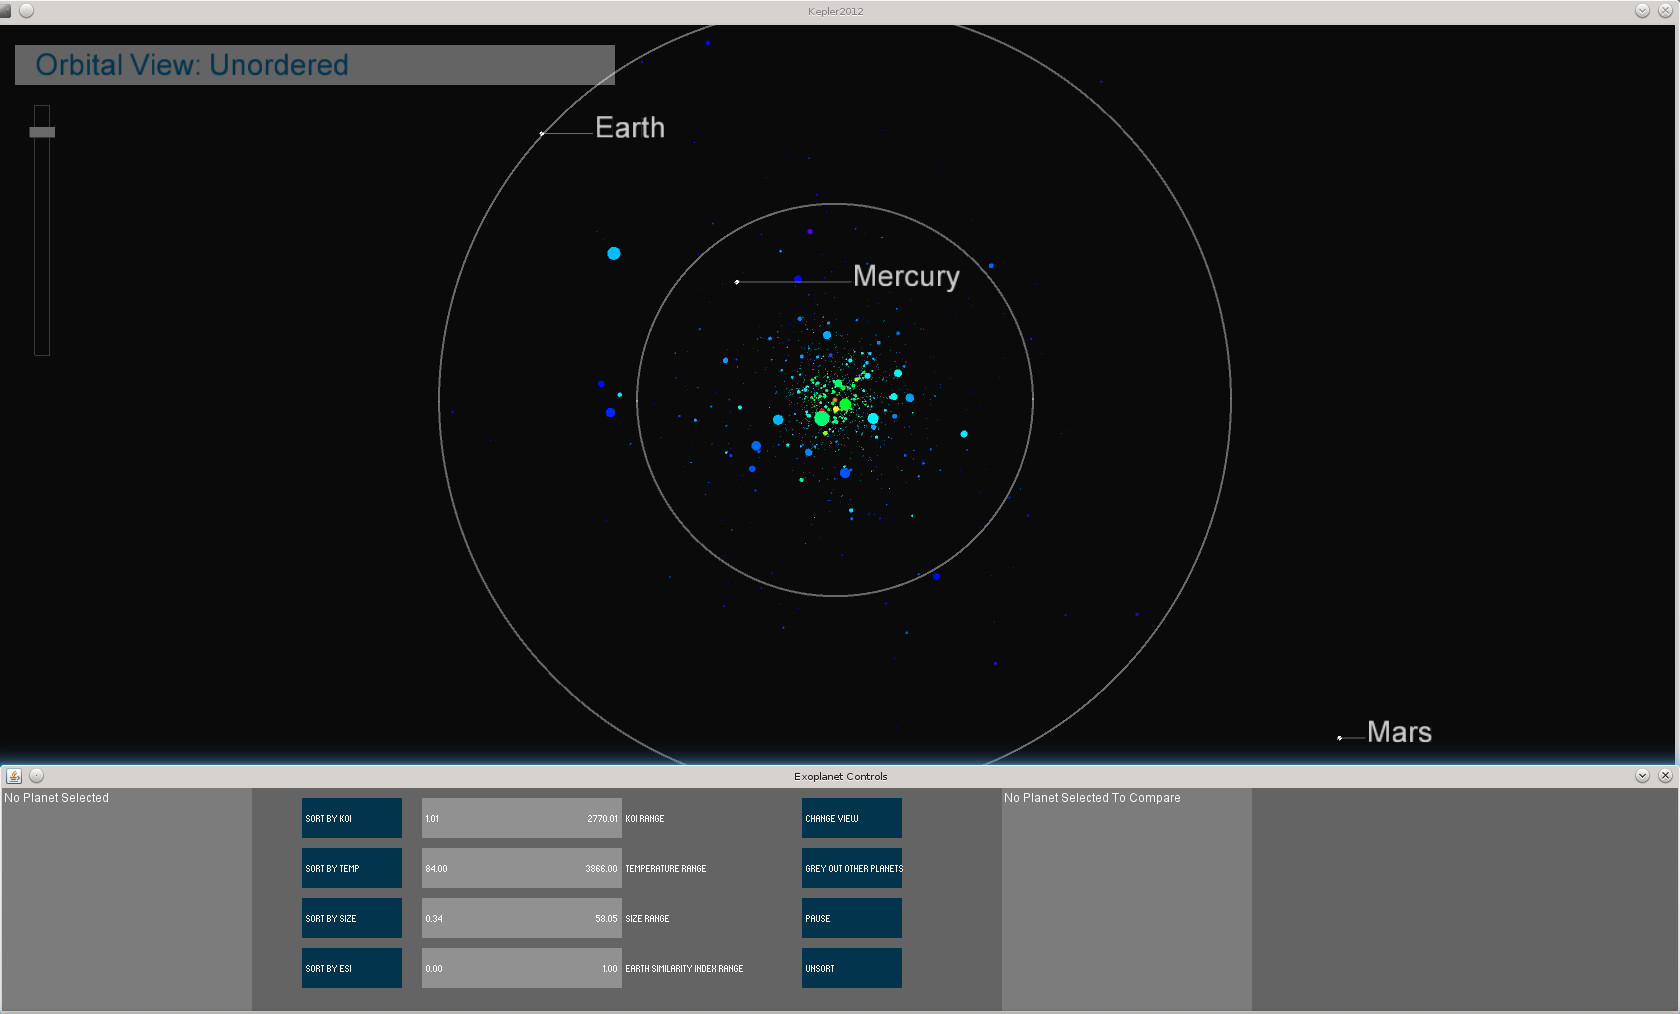
\includegraphics[width=0.8\textwidth]{images/layout_horizontal.jpg}
  \caption{Original Horizontal Layout}  
        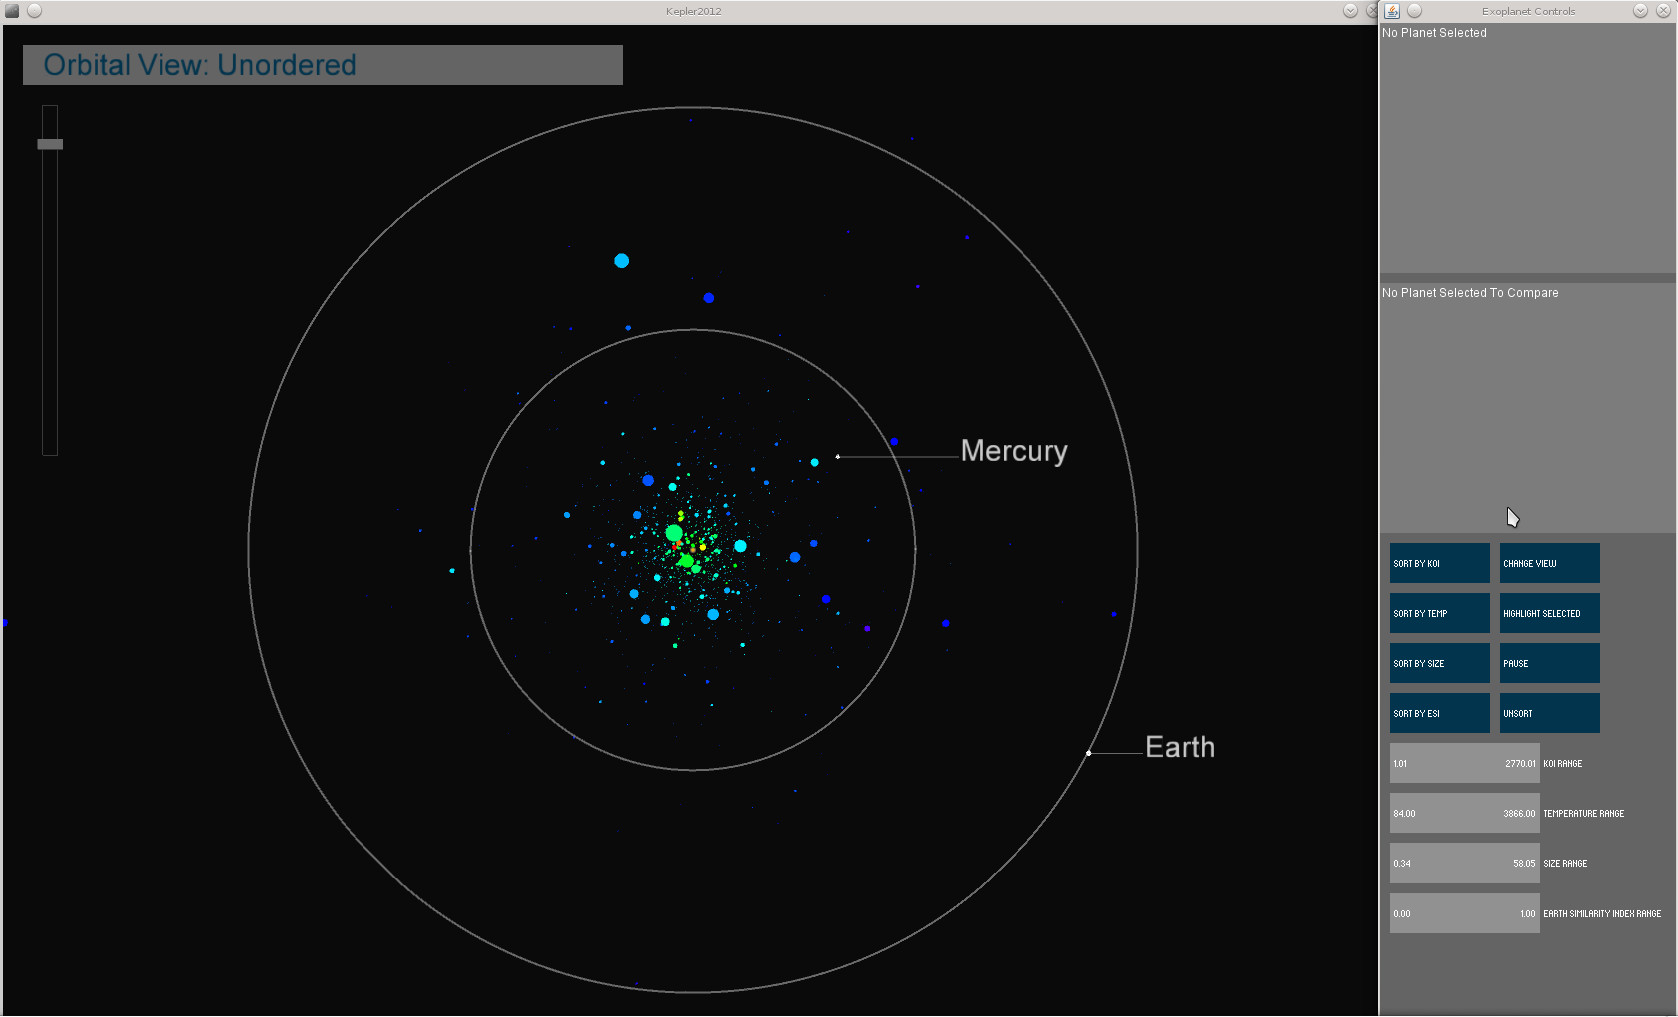
\includegraphics[width=0.8\textwidth]{images/layout_vertical.jpg}
  \caption{Improved Vertical Layout}
\end{figure}

\subsubsection{Navigation Window(BETTER TITLE~)}
Description of navigation window
\begin{figure}[h!]
  \centering
      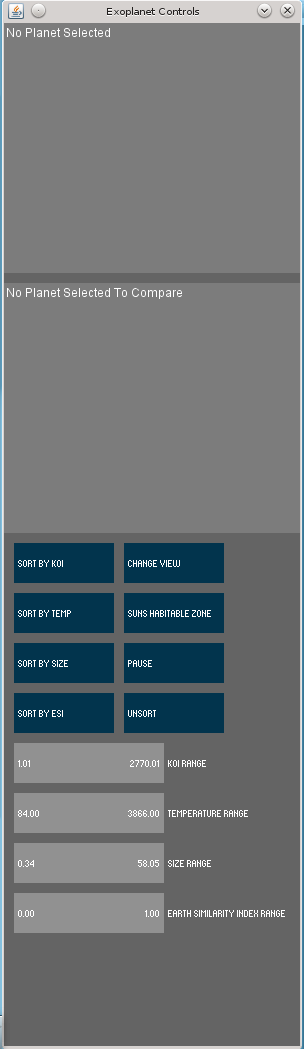
\includegraphics[width=0.3\textwidth]{images/nav.png}
  \caption{Navigation Panel Overview}
  \label{fig:nav}
\end{figure}
Description of each button
\begin{figure}[h!]
  \centering
      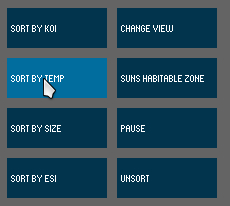
\includegraphics[width=0.6\textwidth]{images/buttons.jpg}
  \caption{Panel of interactive buttons}
  \label{fig:buttons}
\end{figure}
Description of each slider
\begin{figure}[h!]
  \centering
      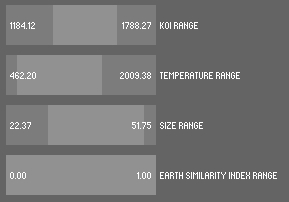
\includegraphics[width=0.6\textwidth]{images/sliders.jpg}
  \caption{Panel of interactive range sliders}
  \label{fig:sliders}
\end{figure}
Description of text boxes
\begin{figure}[h!]
  \centering
      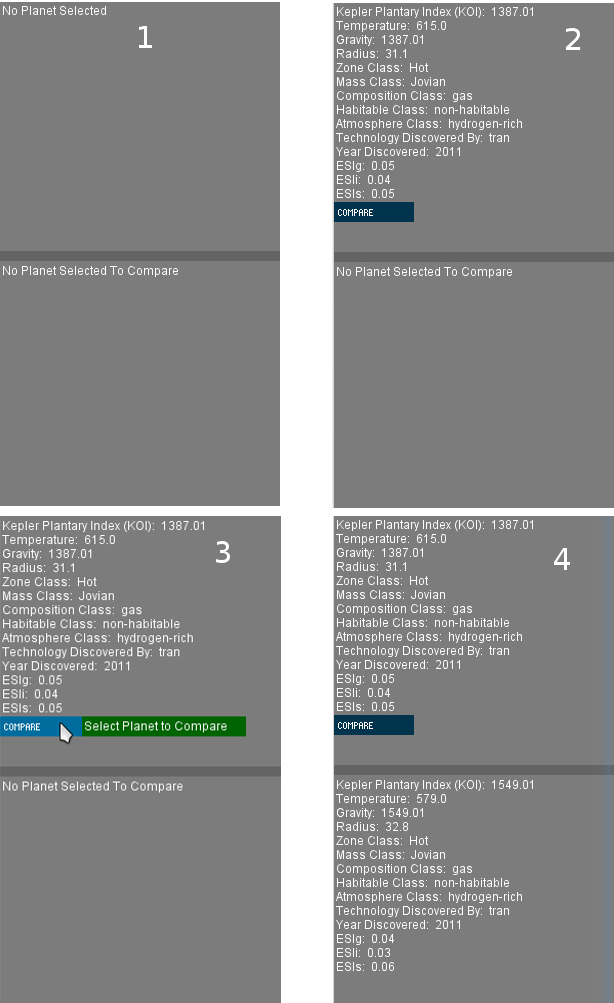
\includegraphics[width=0.9\textwidth]{images/textBoxes.jpg}
  \caption{Text boxes in each possible state}
  \label{fig:sliders}
\end{figure}
Due to the need for increased user interaction with the visualisation a window
is required to house the buttons, range selectors, and text areas. These
elements are needed as the different methods that users can use to interact with
the visualistaion need to be visually apparent to ensure that the system can be
easily used without prior experience. A way to do this is to provide clearly
labelled interactive elements and tooltips explaining what they
do.((REFERENCE))~. These tooltips are widely used as a method of informing a
user about the purpose of an item by hovering over it. This removes the need to
click on a button to discover its effect.

\subsubsection{Visualisation Layout for Kinect sensor}
As the Kinect sensor no longer requires the use of a mouse the visualisation
design needs to be modified to accomodate the use of gestures. For this project
this meant incorporating new cursers to indicate the state of the visualisation.
There are 7 states that the curser needs to be able to be in to inform the user
of what action they are performing. These states are

\begin{enumerate}
 \item default curser, hand is at rest
 \item panning up, hand is raised
 \item panning down, hand is lowered
 \item panning left, hand is to the left
 \item panning right, hand is to the right
 \item zooming in, hand is pressed forward
 \item zooming out, hand is pulled backwards
\end{enumerate}

Having a range of icons that clearly display these states is vital for keeping
the user informed of what they are doing. The icons designed for this purpose
are in the following figure

\begin{figure}[h!]
  \centering
  ~
      %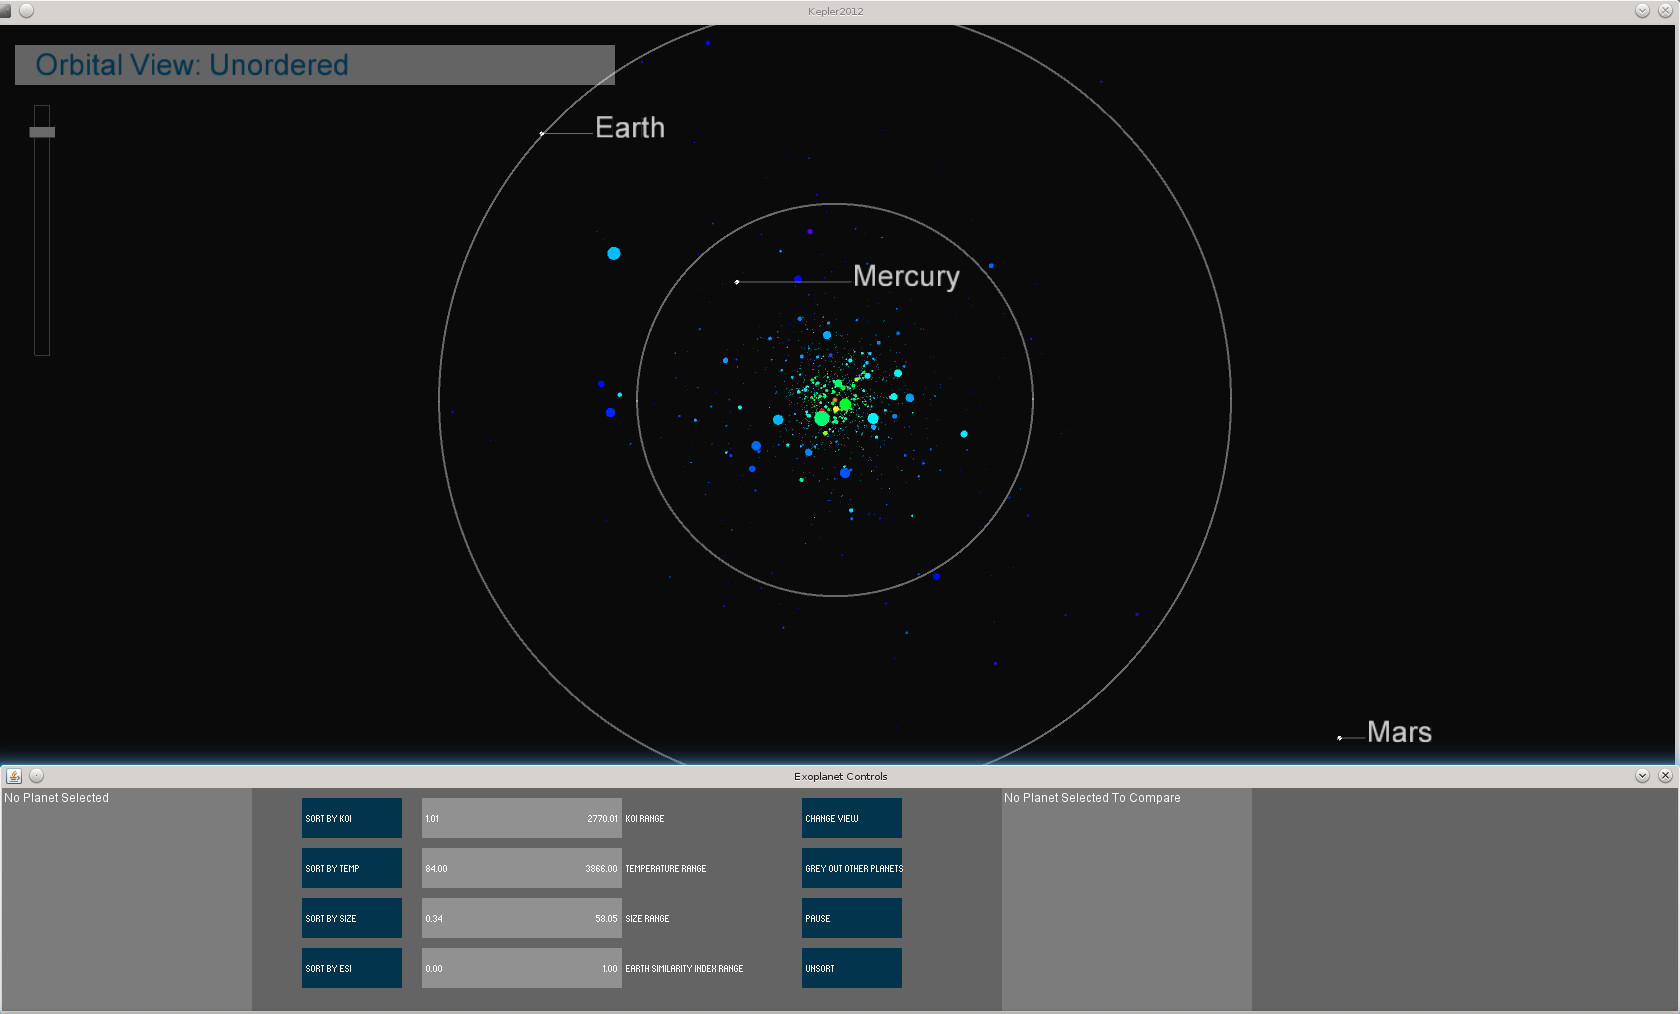
\includegraphics[width=0.8\textwidth]{images/layout_horizontal.jpg}
  \caption{Cursers for Kinect sensor}  
\end{figure}

In addition to this, the screen needs to display the user in relation to the
screen, an effective way to do this is to display a washed out representation of
themselves in the background of the visualisation.
\section{Problems encountered}
Due to the number of elements that needed to be displayed on screen at any one
time (ie 2234 exoplanets), the load placed on a system is very high due to the
need to render 2234 eclipses to represent the planets. This uncovered a bug in
the processing library in which the memory use of the visualisation would
periodically increase until it crashed due to an out of memory exception. After
much experimentation of how to overcome this issue, I discovered that rather
than trying to render a native elipse shape in processing, if I instead rendered
a Scalable Vector Graphic this bug would not manifest. 
\\\\
Libraries used for gesture detection in kinect are opensource in order to work
with processing did not have decent detection
\\\\
Using the Processing framework meant using a non industrial???~ IDE that had
many bugs, for example when undoing multiple times in a row the file being
modified would periodically become corrupted by lines of code being taken away
or inserted into the wrong locations. The solution to this issue was to ensure
that I regularily commited any changes to my version controlled system on Github
((REFERBTECE ~)). Doing this meant that if at any time a file became corrupted I
could easily see the changes in the file when compared against the precious
commit and manually fix the file. 
\\\\
Performance limitations
SCREENSHOT ~

As this project builds upon a previous system much of the existing code and
execution flow needs to be modified. This requires understanding of how the
system was originally built and designed. Because this system does not have any
unit or integration tests, going ahead without a comprehensive knowledge of the
core functionality would be have led to ineffective planning and errors being
introduced into the system.
%Making use of tall of the data
